\subsection{Results of Model Comparisons}
\label{sec:modelres}



\newpage

\subsection{Results of Adaptive Sampling}
\label{sec:adaptiveres}

Define sinusoidal toy model and justify

Explain hyperparameter tests: initsamples, stepsamples, MCMC length

\begin{figure}[h]
    \centering
    \begin{subfigure}[t]{0.5\textwidth}
        \centering
        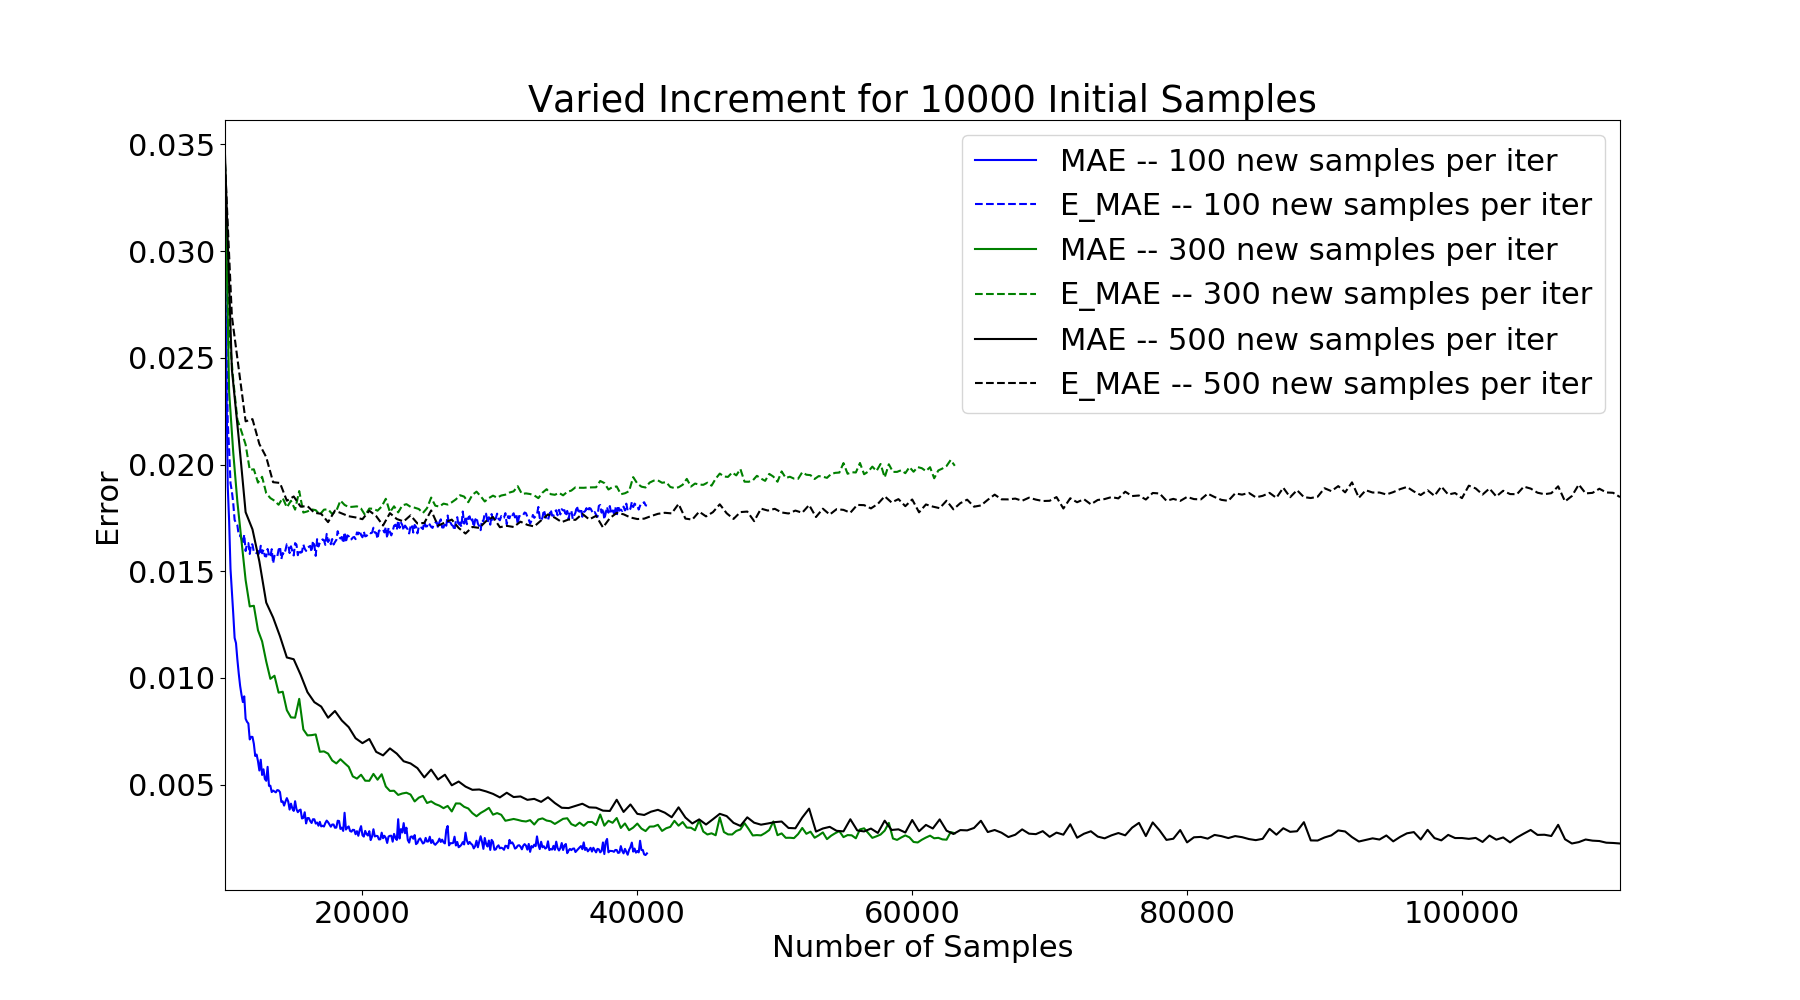
\includegraphics[width=1.1\linewidth]{fig5_qassincrsamp.png}
        \caption{QASS absolute training error over total sample quantity}
    \end{subfigure}%
    ~ 
    \begin{subfigure}[t]{0.5\textwidth}
        \centering
        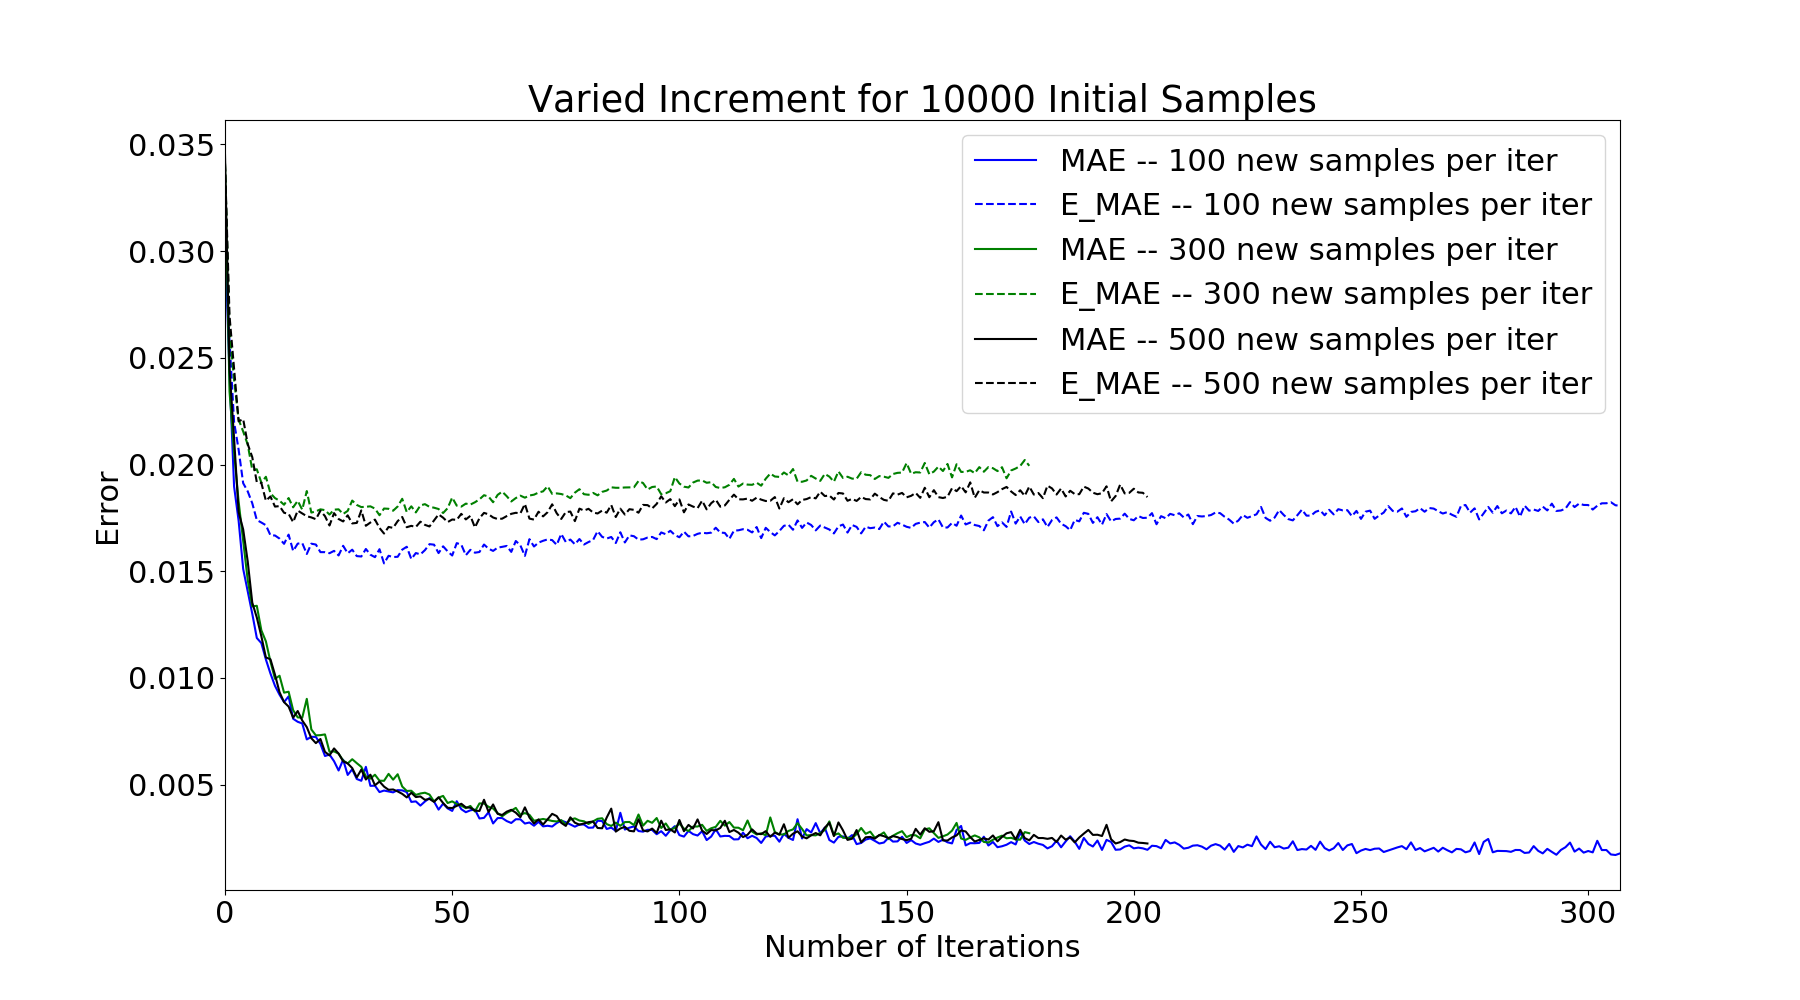
\includegraphics[width=1.1\linewidth]{fig6_qassincrtime.png}
        \caption{QASS absolute training error over number of iterations}
    \end{subfigure}
    \caption{Caption place holder}
\end{figure}

\begin{figure}[h]
  \centering
    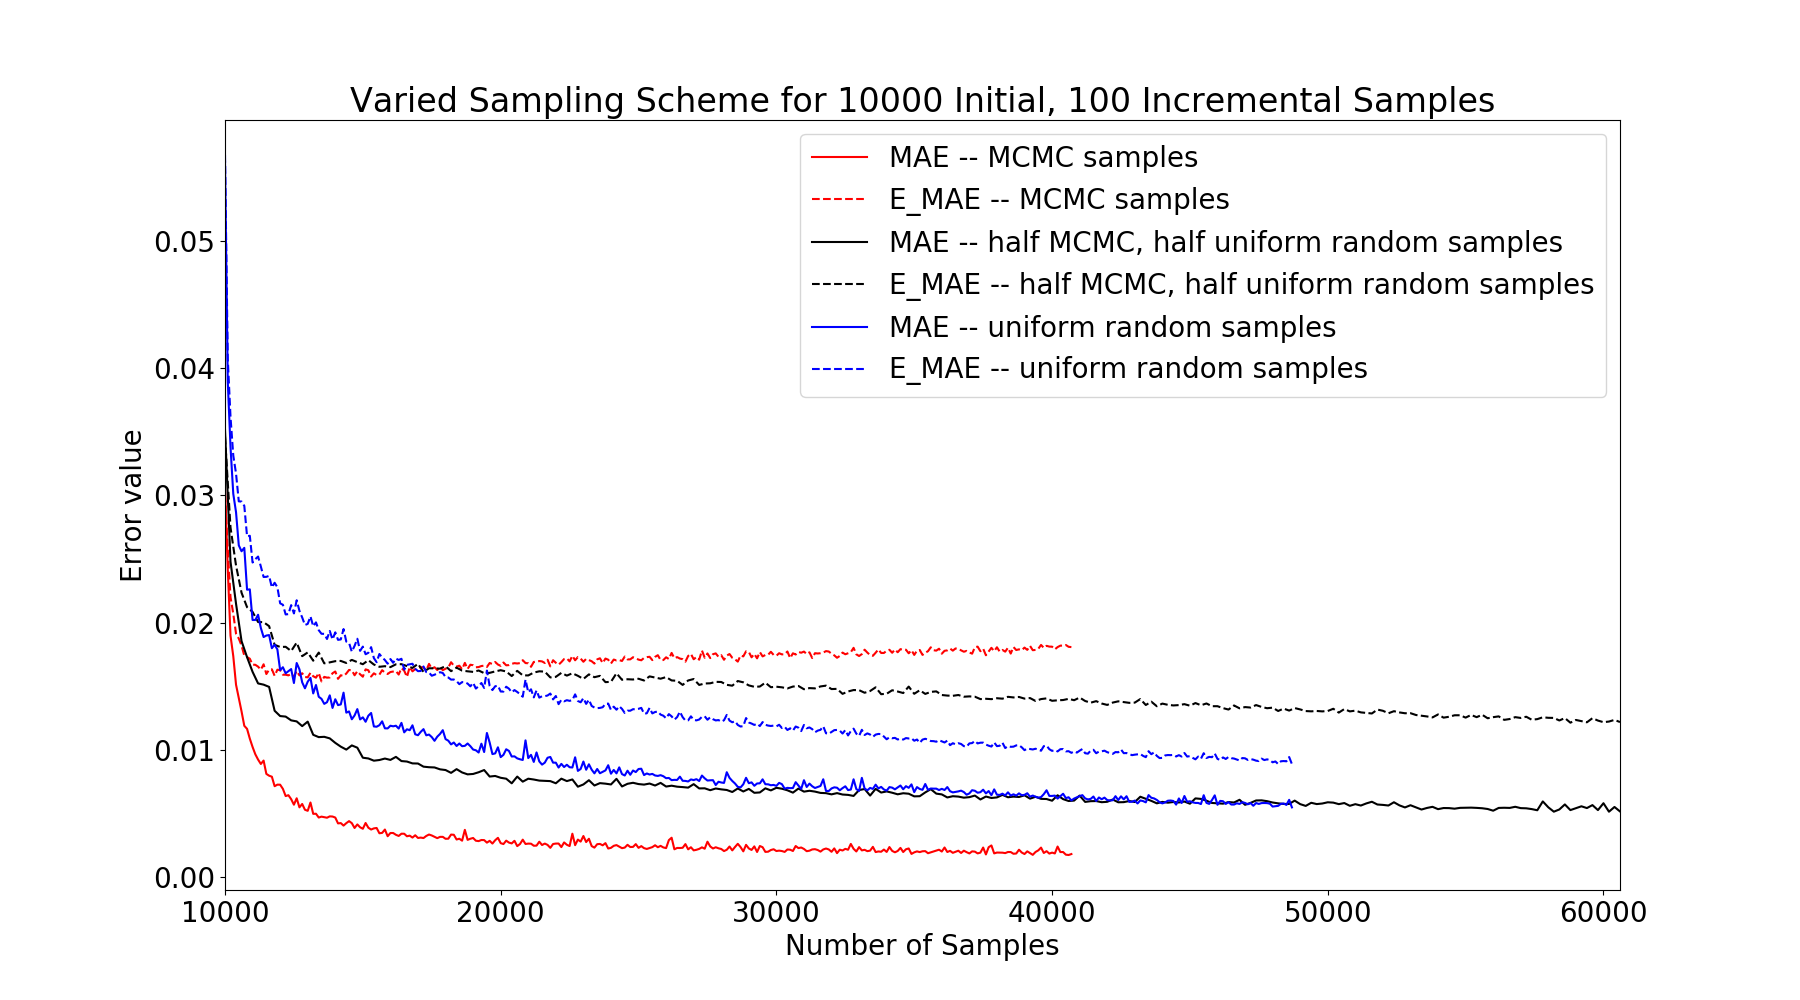
\includegraphics[width=0.8\linewidth]{fig7_qasssampling.png}
    \caption{Absolute training error for QASS, uniform random scheme, and mixed scheme}
  \label{fig:pca}
\end{figure}
